 %!TEX root = demo.tex
\section{Logical Operators}
Now, we discuss the logical operators and their parameterization defined in \projx.

\vspace{0.5em}

\noindent \textsf{SimilarityJoin(R,S,$\phi$, $t$)}: For a given relations $R(a_1,...,a_l)$ and $S(b_1,...,b_k)$, a similarity function $\phi$, and a threshold $t$, the similarity join of R and S is defined by:
\[
\{ (r,s) \in R \times S \text{ s.t } \phi (r,s) \ge t \}
\]

\vspace{0.5em}


\noindent \textsf{Filter(R, $\rho$)}: For a given relation $R(a_1,...,a_l)$ and a boolean condition $\rho$, return $R' \subseteq R$ that satisfies $\rho$.

\vspace{0.5em}

\noindent \textsf{Extract(R, a, $\epsilon$)} For a given relation $R(a_1,...,a_l)$, a attribute $a$, and an extraction function $\epsilon$, apply $\epsilon$ to every $R(a)$ returning $\epsilon(R(a)) = (v_1,...,v_k)$. The result relation is:
\[
R(a_1,...,a_l,\epsilon(R(a)))
\]

\noindent \textsf{Sample(R, $m$)}: For a given relation $R(a_1,...,a_l)$ and return $R' \subseteq R$ such that each $r \in R$ is in $R'$ with probability $m$.

\vspace{0.5em}

\noindent \textsf{Project(R, $p_1,...,p_k$)}: For a given relation $R(a_1,...,a_l)$ and return $R(p_1,...,p_k)$.

\vspace{0.5em}

\noindent \textsf{TransitiveClosure(R,$f$)}: For a given relation of pairs of rows from the same base relation, e.g the result of a self-Similarity Join, $R(a_1,...,a_l, b_1,...,b_l)$ return the transitive closure of the relation $S(a_1,...,a_l)$. $f$ is called a cannonical representation function, this takes a set of associated records and returns a single record that is designated as the canonical representation.

\vspace{1em}

\noindent\textbf{Lineage: }
We track the lineage of rows using a primary key.
Users are not allowed to modify this primary key with any operations.
This allows us to apply operations like transitive closure even after projection since we have a unique identifier for each row.

\vspace{0.5em}
\noindent \textbf{Example: } Suppose, we are interested in deduplication of unstructured data. Then, we could apply the following logical operations.
We first apply an \textsf{Extract} operation to extract the unstructured data into columns. If some of the columns are inconsistent in their representation,
we apply \textsf{Project} to those columns that are inconsistent. We can then take a \textsf{SimilarityJoin} to group rows that are similar, and finally
we resolve those differences with \textsf{TransitiveClosure}.

\section{Optimized Physical Operators}
Now we discuss the physical implementations of these operators.
There are a variety of optimizations and concerns of each of the operators, in this paper, we 
only highlight the main features.

\subsection{Similarity Join} 
\projx provides a library of the following commonly used similarity functions: \textsf{JaccardSimilarity}, \textsf{DiceSimilarity},
\textsf{CosineSimilarity}, \textsf{OverlapSimilarity}, and \textsf{EditDistance}.
The user can select one of these similarity functions.
A naive implementation of a Similarity Join is to take the cartesian product and then filter all pairs of record of similarity greater than $t$.
However, the implemented similarity functions are all symmetric and the similarity function is maximized when $r = p$.
So it suffices to compute a similarity $\theta$-join instead of the full Cartesian product.
We can further add an optimization called prefix filtering to further reduce the number of similarity function evaluations.
In prefix filtering, we prune pairs that cannot possibly meet the threshold $t$ based on the number of tokens that overlap which can be determined with an inverted index.

\subsection{Sampling}
\projx provides different variants of uniform sampling.
We provide Bernoulli sampling (in which flips a ``biased coin" for each row) or hash sampling (which hashes an attribute).
Hash sampling allows for joining sampled relations with foreign key relationships.
On the other hand, Bernoulli sampling is less sensitive to skews and leads to more consistent sample sizes.

\subsection{Transitive Closure}
Similarity Joins can create issues with transitivity.
For example, rowA might be similar to rowB and rowB might be similar to rowC, but rowA might not be similar to rowC.
We can associate these relationships with edges in a similarity graph.
Then to enforce transitive closure, we solve a connected components problem.
We apply a distributed using a distributed gather-apply-scatter connected components algorithm in the Spark-integrated graph library GraphX.

\subsection{Extraction}
We implement basic automated extraction libraries including delimited splitting and regular expression methods.
However, extraction is a task that is well suited for crowd sourcing.
We provide a parametrized interface that allows the user to specify an extraction attribute, a formatting question, and request data from the crowd.
In Figure \ref{fig:entry}, we illustrate an example of this task.

\begin{figure}[ht!]
\centering
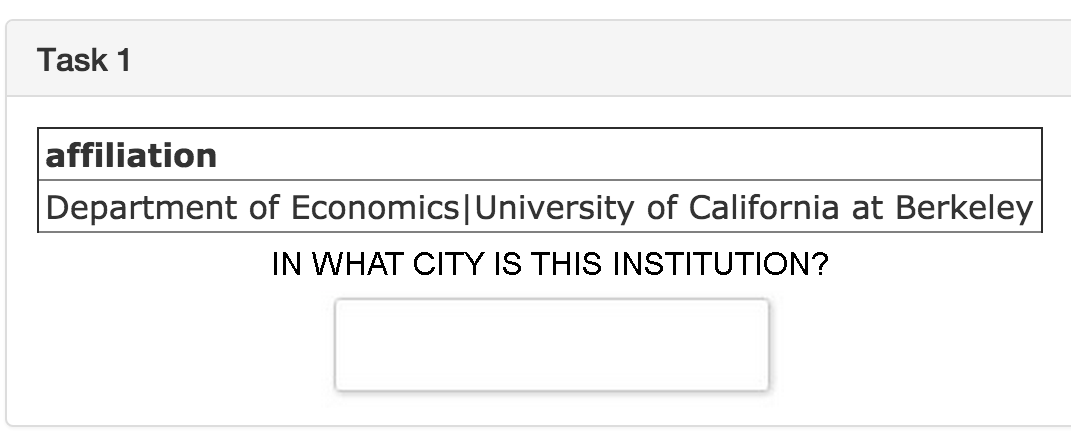
\includegraphics[scale=0.25]{figs/entry.png}
\caption{Example of the Extraction Crowd Interface. \label{fig:entry}}\vspace{-.5em}
\end{figure}

\subsection{Filtering}
We provide an interface for a user defined predicate.
However, as with extraction, filtering has many opportunities for crowdsourcing.
For a filtering operation, the crowd response is binary in contrast to Extraction.
We provide crowd templates for two types of filtering tasks.

\noindent\textbf{Condition Checking: } Given a single record, a crowd worker indicates if it satisfies some condition. In Figure \ref{fig:condition},
we illustrate an example condition checking task.
\begin{figure}[ht!]
\centering
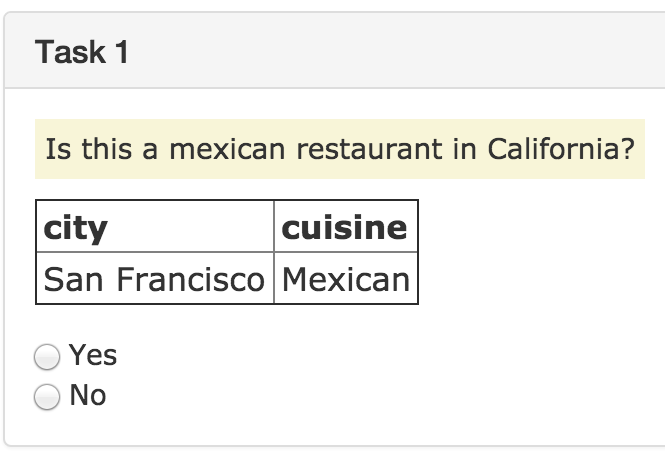
\includegraphics[scale=0.25]{figs/condition.png}
\caption{Condition checking is one variant of the filtering crowd interface.\label{fig:condition}}\vspace{-.5em}
\end{figure}

\noindent\textbf{Pair Comparison: } Given a pair of records, a crowd worker indicates if they are the same or are different. In Figure \ref{fig:pair},
we illustrate an example pair comparison task.

\begin{figure}[ht!]
\centering
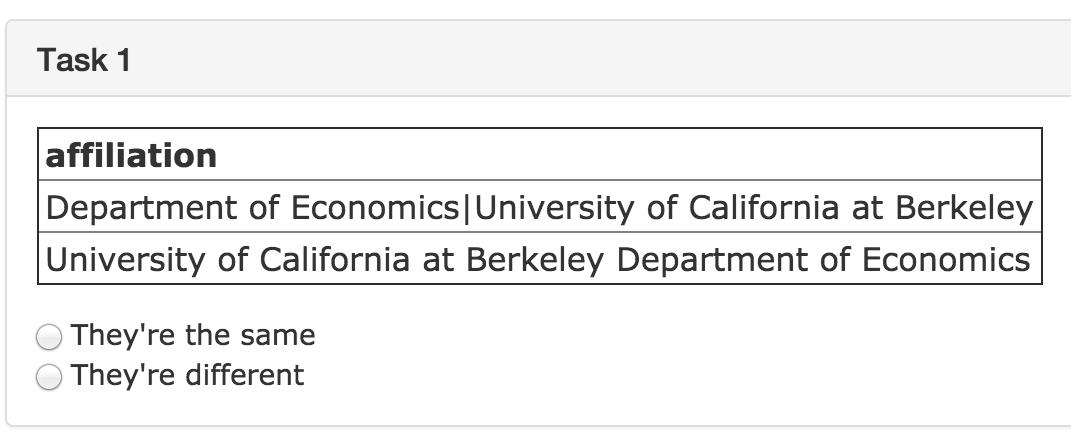
\includegraphics[scale=0.25]{figs/pair.png}
\caption{Pair comparison is the other variant of the filtering crowd interface.\label{fig:pair}}\vspace{-.5em}
\end{figure}

\subsection{Learning Parameters From Example}
In simple cases, it might be easy to use domain knowledge to select and tune physical operators. 
In more complex cases, it might be easier to specify a sample of dirty and clean data instead of the function.
It may also not be feasible to have the crowd clean the entire dataset.
In these cases, we want to learn a statistical model from which we can extrapolate those responses to the rest 
of the data.

In our current implementation of \projx, we pose this learning problem as classification problems.
In general, these parameter functions can be quite complex and this is a simplification of the learning problem.
The choice of classifier and featurization is upto the user. 
We currently support Support Vector Machines and Decision Trees with a featurization library that includes common text processing features.

\vspace{0.5em}

\noindent \textsf{Filter(R, $\mathcal{T}^+$, $\mathcal{T}^-$)}: Given a set of positive training examples $\mathcal{T}^+$ (i.e, $r$ that satisfy the condition) and
negative training examples $\mathcal{T}^-$ (i.e, r that do not satisfy the condition), we learn a classifier that predicts whether a record satisfies the condition. 

\vspace{0.5em}

\noindent \textsf{Extract(R, a, $\mathcal{T}$)} We restrict the learned problem setting to delimited extraction. Given a set of training examples $R(a)$ and the output $v_1,v_2,...,v_k$, we learn a classifier to predict which characters in $R(a)$ are delimiters based on the tokens in the string.

\vspace{1em}

To acquire the samples of clean data, uniform sampling may not be the best strategy.
For example, if there examples of dirty data are very rare, we will not be able to learn a model.
We implement a technique called Active Learning to sample.
Active Learning selects the most informative examples based on the current model so far.
We use an Active Learning algorithm called uncertainty sampling to do this.








